\chapter{Navigation}
\section{Bekanntes vs. unbekanntes Terrain}
Man unterscheidet zwischen Algorithmen für:
\begin{itemize}
	\item \textbf{bekannte Umgebungen} (auch während der Fahrt ändert sich die Umgebung nicht)
	\item \textbf{unbekannte Umgebungen}
\end{itemize}
\begin{itemize}
	\item Gebiet \textbf{vollständig bekannt} $\Rightarrow$ Lösung der Suche mittels eines Graphen.
	\item \textbf{unvollständig oder gar nicht bekanntes Gelände} $\Rightarrow$ Berechnungen erfolgen auf \textbf{lokalen Teilinformationen}
	\subitem Neue Informationen $\Rightarrow$ \textbf{inkrementelle Anpassung} über Sensoren
\end{itemize}
\section{Navigation in unbekanntem Terrain}
\subsection{Konturverfolgung}
\begin{itemize}
	\item Eine \textbf{Freiraumfahrt} d.h. eine Fahrt durch ein Gelände, dessen Raum möglichst weit und frei von Hindernissen ist $\Rightarrow$ nicht immer Zielführend
	\item Lösung: \textbf{Konturverfolgung}
	\subitem Roboter wird nah an einem Objekt (Wand, Hinderniss) entlang bewegt
	\subitem Es sollte möglichst ein gegebener Abstand $d$ eingehalten werden
\end{itemize}
\paragraph{Regelung des Abstands d}
\begin{lstlisting}
IF (Distance to Wall > d) 
	THEN turn to wall

IF (Distance to Wall < d) 
	THEN turn away from wall

IF (Distance to Wall == d) 
	THEN Drive straight ahead
\end{lstlisting}
\newpage
\subsection{Sensorbasierte Planer - Navigation mit Hinderniskontakt}
\subsubsection{Bug1 Algorithmus}
Fordert zwei bestimmte Verhalten:
\begin{itemize}
	\item bewege dich auf einer geraden Linie
	\item folge einer Begrenzung in einem bestimmten Abstand
\end{itemize}
\begin{figure}[H]
	\begin{center}
		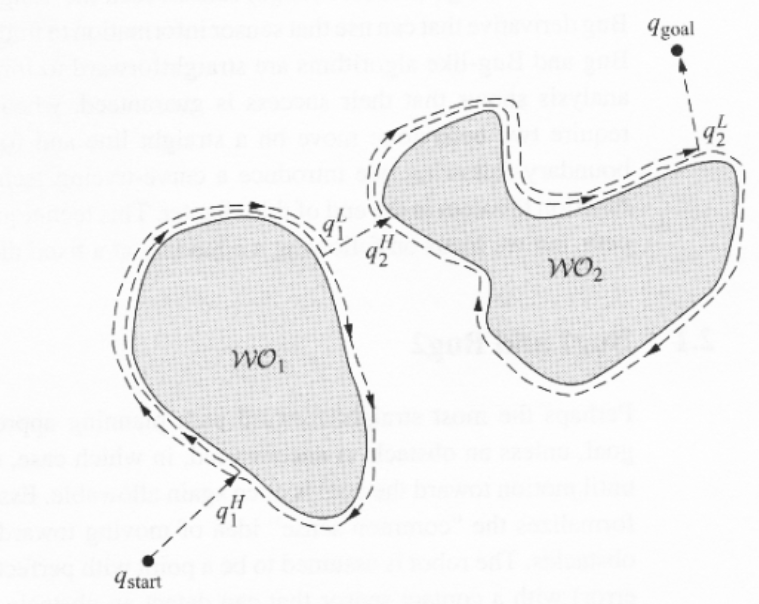
\includegraphics[scale=0.5]{Resources/PNG/Bug1.png}
		\caption{Bug1 Algorithmus Route}
		\label{fig:PNG/Bug1.png}
	\end{center}
\end{figure}
\paragraph{Vorraussetzungen}
\begin{itemize}
	\item Roboter benötigt einen Sensor zur Erkennung eines \enquote{Kontakts} mit einem Hindernis
	\item Roboter kann die Distanz zwischen zwei Punkten x und y messen
	\item der Arbeitsraum ist begrenzt
\end{itemize}
\paragraph{Algorithmus}
\begin{itemize}
	\item Roboter folgt Linie zum Ziel bis er beim Punkt $q_1^H$ auf ein Hinderniss trifft
	\item Roboter umfährt das Hindernis bis er erneut beim gleichen Punkt auf das Hindernis trifft
	\item Roboter bestimmt den nähesten Punkt (Leavepoint) $q_1^L$ vom Hindernis zum Ziel und fährt diesen Punkt an
	\item Von diesem Punkt fährt der Roboter geradewegs zum Ziel bis er das Ziel erreicht oder erneut auf ein Hindernis trifft
\end{itemize}
\paragraph{Exception}
Schneidet die Linie von $q1^L$ zum Ziel das \textbf{aktuelle Hindernis} gibt es keine Lösung
\begin{figure}[H]
	\begin{center}
		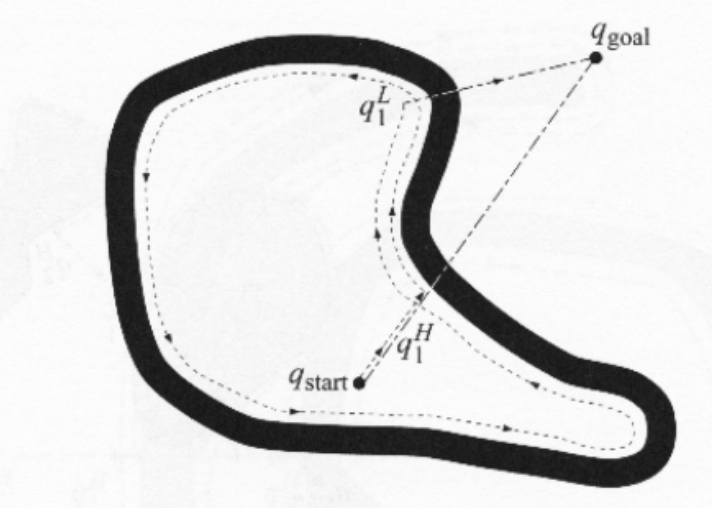
\includegraphics[scale=0.4]{Resources/PNG/Exception1.PNG}
		\caption{}
		\label{fig:PNG/Exception1.PNG}
	\end{center}
\end{figure}
\subsubsection{Bug2-Algorithmus}
\textbf{Idee:}
\begin{itemize}
	\item Linie vom Start $S$ zum Ziel $T$ konstruieren
	\item bewegt sich möglichst auf dieser Linie
	\item Roboter trifft auf Objekt $\Rightarrow$ umfahren in einer bestimmten Richtung bsp. immer rechts herum
	\item Hindernis wird solange umfahren, bis der Roboter wieder auf einen Punkt auf der Linie $ST$ trifft, der näher zum Ziel liegt als der ursprüngliche Kontaktpunkt mit dem Hindernis
\end{itemize}
\textbf{Algorithmus}:
\begin{lstlisting}
1. Auf Geraden ST in Richtung T fahren bis:
	a.) Ziel erreicht wird --> END
	b.) Hinternis getroffen wird --> Schnittpunt Hj setzen
		--> Schritt 2
2. Umfahre das Objekt bis:
	a.) das Ziel erreicht wird --> END
	b.) Gerade ST in einem Punkt Q getroffen wird mit Strecke QT kleiner als Strecke HjT
		QT wird in Richtung T verlassen
		Q als Leavepount Lj setzen
		i um 1 erhoehen
		--> Schritt 1
	c.) zum letzten Hitpoint Hj zurueckgekehrt wird
		Algorithmus wird abgebrochen
		Es gibt keinen Weg zu T
\end{lstlisting}
\begin{itemize}
	\item Ev. wird kein Weg zum Ziel gefunden
\end{itemize}
\begin{itemize}
	\item Bei Komplexen Hindernissen kann Ziel mit \textbf{Backtracking} gefunden werden
\end{itemize}
\subsubsection{Bug3-Algorithmus}
\begin{figure}[H]
	\begin{center}
		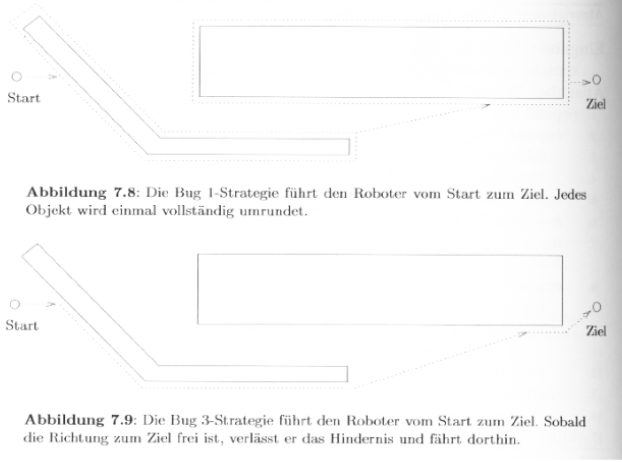
\includegraphics[scale=0.6]{Resources/PNG/Bug3.PNG}
		\caption{}
		\label{fig:PNG/Bug3.PNG}
	\end{center}
\end{figure}
\subsection{Labyrinthe}
\paragraph{Grundprobleme}
\begin{itemize}
	\item Es wird davon ausgeangen, dass der Roboter berühren oder \enquote{sehen} kann
	\item Zwei grundlegend Hauptprobleme:
	\subitem Einen \textbf{Weg in ein Labyrinth} finden, um einen bestimmten Gegenstand oder \textbf{Schatz zu erreichen} sowie den \textbf{Rückweg zum Eingang}
	\subitem \textbf{Flucht aus einem Labyrinth} von einer unbekannten Stelle aus.
	\item Enger Zusammenhang zwischen Labyrinth und Graphen $\Rightarrow$ Jeder Korridor:= Kante und jede Kreuzung:= Knoten
	\subitem Bei bekanntem Labyrinthe $\Rightarrow$ Suchproblem auf in Bäumen
\end{itemize}
\paragraph{Verlassen eines Labyrinths mit Pledge Algorithmus}
\textbf{Grundidee}: Vorsichtig geradeaus bis man auf ein Hindernis trifft und dann mit der \enquote{linken} Hand immer an der Wand entlang bis zum Ausgang.\\
\textbf{Problem}: Enthält das Labyrinth eine Säule, läuft man für immer im Kreis
\begin{itemize}
	\item \textbf{Lösung} $\Rightarrow$ man folgt der Wand nur solange, bis man wieder in die alte Richtung schaut.
\end{itemize}
\textbf{Allgemeingültige Lösung}: Drehungen beim Abbiegen an den Ecken mitzählen.
Bei jeder Linksdrehung wird der Umdrehungszähler inkrementiert, bei jeder Rechtsdrehung dekrementiert.
\begin{itemize}
	\item Bewege den Roboter geradeaus bis eine Wand erreicht ist
	\item Folge der Wand bis Umdrehungszähler 0 ist
\end{itemize}
\paragraph{Verlassen eines Labyrinths mit Ariadenfaden}
\begin{itemize}
	\item \textbf{Ziel}: einen Weg zu einem versteckten Ziel im Labyrinth sowie wieder zurück zum Eingang finden ohne dass eine Karte des Labyrinths bekannt ist
	\item \textbf{Idee}: Wenn man ein Labyrinth betritt Faden ausrollen $\Rightarrow$ zurückverfolgen bringt einen zurück zum Eingang.
\end{itemize}
\textbf{Vorraussetzungen und grundsätzliches Vorgehen}
\begin{itemize}
	\item einer Wand folgen
	\item Umdrehen
	\item Kreuzungen erkennen
	\item Ziel erkennen
	\item Faden auslegen und wieder einsammeln
	\item Faden am Boden erkennen
	\item Faden zur nächsten Kreuzung folgen
\end{itemize}
\paragraph{Tarry und Tremaux Algorthmus}
\begin{itemize}
	\item Beispiel für klassische Tiefensuche
	\item Richtung, in der sich das zu suchende Objekt befindet ist unbekannt.
	\item Graph kann zyklen enthalten
	\item Es wird ein zyklisch gerichteter Graph durch jede Kante konstruiert, wobei jede Kante nur einmal pro Richtung besucht wird
\end{itemize}
\textbf{Algorithmus:}
\begin{itemize}
	\item Starte willkürlich an einem Knoten
	\item Folge einem möglichen Pfad, markiere die Kante, in welcher Richtung sie betreten worden ist
	\item Sind alle Kanten schon betreten, eine auswählen, die bis jetzt nur in die Gegenrichtung betreten wurde.
	\item Trifft man auf eine Sackgasse oder einen schon besuchten Gang, zurück zur letzten Kreuzung
	\item Es darf kein Pfad betreten werden, der schon in beide Richtungen besucht wurde.
	\item Algorithmus ist beendet, wenn der Startpunkt erreicht wird.
\end{itemize}
\section{Pfadplanung für mobile Roboter in bekanntem Terrain}
\subsection{Bewegungsplan für mobile Roboter}
Ziel der Navigation ist es, ein Fahrzeug in der Umwelt zu bewegen.
Dies beinhaltet drei Unteraufgaben:
\paragraph{Globale Pfadplanung}
\begin{itemize}
	\item \textbf{Vorraussetzung}: es gibt eine Karte
	\item suche eines Pfades von einem Start- zu einem Zielpunkt in vorhandenem Umgebungsmodell
	\item evtl. auch Suche nach Pfad mit geringsten Kosten
	\item Kompletter Pfad beschrieben durch Menge von Punkten
\end{itemize}
\paragraph{Lokale Pfadplanung} berücksichtigt Fahrzeug-Dimension und kinematische Einschränkungen
\paragraph{Path Control} generiert geeignet Steuerbefehle, um den vorberechneten Pfad zu folgen
\subsection{Konfigurationsraum}
\paragraph{Herleitung}
\begin{itemize}
	\item Abmesungen, Form, Bewegungsmöglichkeiten des Roboters werden für die Erstellung des Konfigurationsraums benötigt
	\item Konfiguration $q$ eines Roboters beschreibt Lage und Ausrichtung im Bezugssystem des Umgebungsmodells
	\item Im zweidimensionalen Raum kann Position in $x,y$-Ebene und Orientierung ausgedrückt werden
	\item Konstruktionsbedingt sind einige Konfigurationen für den Roboter in seiner Umgebung nicht zulässig
	\item Problem; einfachere Darstellung:
	\subitem Roboter als Punkt angenommen
	\subitem Abmessungen des Roboters + Objektabmessungen $\Rightarrow$ Konfigurations-Hindernisse
\end{itemize}
\begin{figure}[H]
	\begin{center}
		\includegraphics[scale=0.5]{Resources/PNG/Konfigurationshindernisse.PNG}
		\caption{}
		\label{fig:PNG/Konfigurationshindernisse.PNG}
	\end{center}
\end{figure}
\paragraph{Definition}
\begin{itemize}
	\item Summe aller Konfigurations-Hindernisse bildet den \textbf{Konfigurationsraum}
	\item Konfigurationsraum ist Datenstruktur, die es dem Roboter ermöglicht, die Position und Orientierung von Hindernissen in der Umgebung zu definieren
	\item Der Konfigurationsraum dient als Basis der Wegplanung
\end{itemize}
\paragraph{Repräsentationen}
\begin{itemize}
	\item Graphen mit Knoten
	\item Reguläre Gitter
	\item Quad-Bäume oder Octal-Bäume oder als Voronoidiagramme
\end{itemize}
\section{Algorithmen und Methoden}
Für die folgenden Algorithmen und Methoden wird ausgeganen, dass Hindernisse bekannt sind und weder Position noch Form ändern
\paragraph{Zellzerlegungen} das Umgebungsmodell wird in sich nicht überlappende Zellen unterteilt, die als besetzt oder frei markiert sind
\paragraph{Roadmaps}
\begin{itemize}
	\item Das entstehende Netzwerk muss \textbf{topologisch} alle zwischen den Hindernissen befahrbare Wege umfassen.
	\item Planer kann dann kollisionsfreien Pfad von Start- zu Zielpunkt erstellen
\end{itemize}
Auf dieses Netzwerk können Standardmethoden der Graphentheorie, wie sie auch in der Autonavigation Verwendung finden, andwendet werden:
\begin{itemize}
	\item kürzeste Wegsuche mit A*, Dijkstra
	\item Wegsuche mit Umgehung von Hindernissen mit dem \textbf{Sichtbarkeitsgraph}
	\item Wegsuche mittels eines \textbf{Voronoigraphen}, \textbf{Voronoidiagramms}
\end{itemize}
\paragraph{Potentialfeldmethoden} beinhalten die physikalische Simulation des Roboters als Partikel in einem Feld.
\newpage
\subsection{Dijkstra}
%\paragraph{Datenstrukturen}
%\begin{itemize}
%	\item \textbf{PriorityQueue} $Open$
%	\item \textbf{Aktueller Knoten} $n$
%	\item \textbf{Nachfolgerknoten} $n'$
%	\item \textbf{Vorgänger} $predecessor$
%	\item \textbf{Startknoten} $s$
%	\item \textbf{Kosten} $cost$
%\end{itemize}
\paragraph{Funktionsweise}
\begin{enumerate}
	\item Alle Knoten werden als \textbf{unbesucht} markiert $\Rightarrow$ kreiert ein set namens \textbf{unbesuchtes Set}
	\item Allen Knoten wird ein \textit{temporärer Distanzwert} zugeordnet.
	\subitem Ursprungsknoten := 0
	\subitem Alle anderen Knoten := $\infty$
	\item Setzen des Ursprungsknoten als \textit{current} Knoten
	\item Für den \textit{current} Knoten alle \textit{unbesuchten} Nachbarn betrachten und deren \textit{temporären Distanzwert berechnen}.
	Vergleichen des \textit{temporären Distanzwert} mit dem \textit{jetzigen Distanzwert} innerhalb des Nachbarknotens.
	Falls der temporäre Distanzwert kleiner ist als der jetzige Distanzwert innerhalb der nachbarn wird der temporäre Distanzwert eingetragen.
	\item Sobald alle Nachbarn überprüft wurden und alle werte eingetragen sind, wird der betrachtete Knoten auf \textbf{besucht} gesetzt. Somit wird er aus dem angelegten Set entfernt und wird nicht mehr überprüft.
	\item Sobald der Zielknoten als besucht markiert ist dann terminiert der Algorithmus, \textbf{else} wird der Knoten mit der niedrigsten temporären als neuer \textbf{current} Knoten gesetzt und schritt 4 wird wiederholt.
\end{enumerate}

%TODO Algorithmus
\subsection{A*}
%\paragraph{Datenstrukturen}
%\begin{itemize}
%	\item \textbf{PriorityQueue} $Open$
%	\item \textbf{List} $Closed$
%	\item \textbf{Aktueller Knotne} $n$
%	\item \textbf{Nachfolgerknoten} $n'$
%	\item \textbf{Vorgänge} $predecessor$
%	\item \textbf{Startknoten} $s$
%	\item \textbf{Kosten} $g = bekannte Kosten$, $h = Schätzkosten$, $f = Gesamtkosten$
%\end{itemize}
\paragraph{Funktionsweise}
%TODO Algorithmus
\subsection{Wegsuche mit dem Sichtgraph-Algorithmus}
\paragraph{Visibility Map}
\begin{itemize}
	\item enthält Eckpunkte von Polygonen, den Ecken der Hindernisse
	\item zwei Knoten der Visibility Map teilen eine Kante, wenn die beiden Eckpunkte voneinander in Sichtweite sind
\end{itemize}
\paragraph{Visibility Graph}
\begin{itemize}
	\item ist die einfachste Visibility Map
	\item Knoten umfassen: \textbf{Startknoten}, \textbf{Zielknoten} und alle Eckpunkte der Hindernisse
	\item die Kanten sind Liniensegmente, die zwei Knoten in Sichtweite verbinden
	\item Hinderniskanten sind Teil des Sichtgraphen
\end{itemize}
\paragraph{Sichtgraphenalgorithmus}
\begin{itemize}
	\item verbinde \textbf{Start-}, \textbf{Zielpunkte} und die \textbf{Ecken} der Hindernisse durch Geraden, die nicht durch Hindernisse laufen dürfen
	\item Ergebnis ist ein Graph, dessen Knoten Orte sind und dessen Kanten mögliche Wegstücke zwischen diesen Knoten darstellen
	\item Kanten sind gewichtet mit der Entfernung zwischen den Knoten
	\item gesucht: Menge der möglichen Geraden, die den Startpunkt auf dem kürzesten Weg mit dem Zielpunkt verbindet
	\item \textbf{Nachteil}: führt unmittelbar an Hindernissen entlang, enthält noch viele nutzlose Kanten
\end{itemize}
\begin{figure}[H]
	\begin{center}
		\includegraphics[scale=0.5]{Resources/PNG/Sichtgraphalgorithmus.PNG}
		\caption{}
		\label{fig:PNG/Sichtgraphalgorithmus.PNG}
	\end{center}
\end{figure}
\paragraph{Reduzierter Visibility Graph}
Definition von \textbf{unterstützenden} und \textbf{trennenden} Kanten:
\begin{itemize}
	\item \textbf{unterstützende Kante:} Tangente zu zwei Hindernissen, so dass die Hindernisse auf derselben Seite der Linie liegen
	\item \textbf{trennende Kante:} Tangente zu zwei Hindernissen, so dass die Hindernisse auf gegenüberliegenden Seiten der Tangente liegen
\end{itemize}
Der reduzierte Sichtgraph besteht nur aus unterstützenden und trennenden Kanten.
\begin{figure}[H]
	\begin{center}
		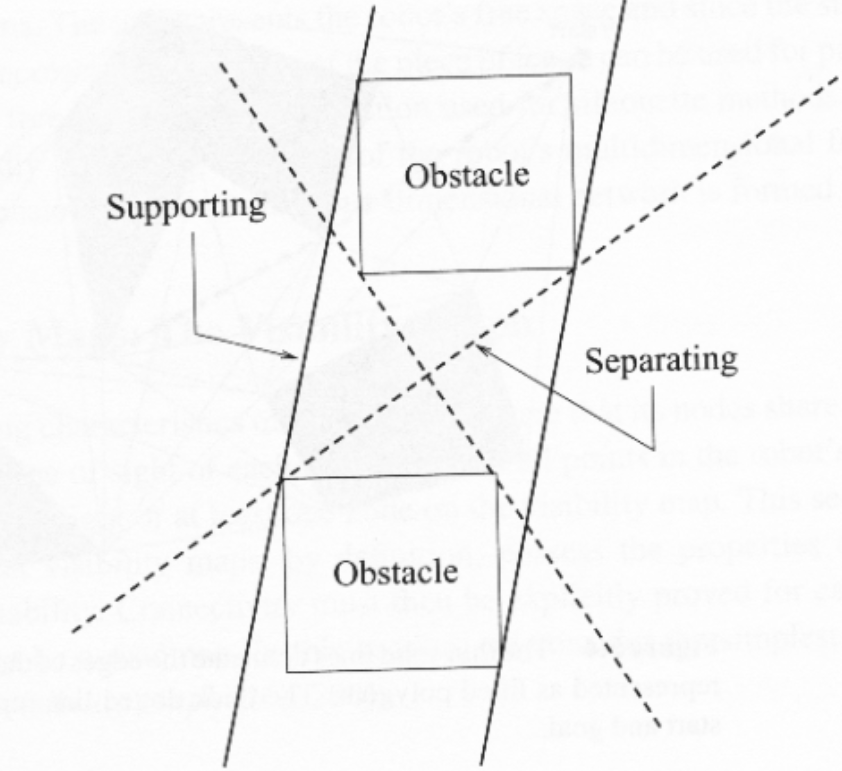
\includegraphics[scale=0.4]{Resources/PNG/SichtGraphReduziert}
		\caption{}
		\label{fig:PNG/SichtGraphReduziert.PNG}
	\end{center}
\end{figure}
\paragraph{Konstruktion des Graphen}
\begin{itemize}
	\item Alle Liniensegmente $vv_i$ mit $v != v_i$ müssen getestet werden, ob sie keinen Schnittpunkt mit einer Kante eines Hindernisses haben
	\item \textbf{Nachteil}: Komplexität O($n^3$)
	\item \textbf{Effizienter}: Plane Sweep Algorithmus mit Komplexität O($n^2 log n$)
\end{itemize}
\paragraph{Algorithmus}
\begin{itemize}
	\item \textbf{Input}: A  set of vertices ${v_i}$ (whose edges do not intersect) and a vertex $v$
	\item \textbf{Output}: A subset of vertices from ${v_i}$ that are within line of sight of $v$
\end{itemize}
\begin{itemize}
	\item For each vertex $v_i$, calculate $\alpha$, the angle from the horizontal axis to the line segment $\overline{vv_i}$
	\item Create the vertex list $\epsilon$, containing the $\alpha_i$'s sorted in increasing order.
	\item Create the active list $\mathcal{S}$, containing the sorted list of edges that intersect the horizontal half-line emanating from v.
	\item \textbf{For all} $\alpha_i$ \textbf{do}
	\subitem if $v_i$ is visible to $v$ \textbf{then}
	\subsubitem Add the edge ($v, v_i$) to the visibility graph.
	\subitem \textbf{end if}
	\subitem \textbf{if} $v_i$ is the beginning of an edge, E, not in $\mathcal{S}$ \textbf{then}
	\subsubitem Insert the \textit{E} into $\mathcal{S}$
	\subitem \textbf{end if}
	\subitem \textbf{if} $v_i$ is the end of an edge in $\mathcal{S}$ \textbf{then}
	\subsubitem Delete the edge from $\mathcal{S}$
	\subitem \textbf{end if}
	\item \textbf{end for}
\end{itemize}
\subsection{Voronoi-Diagramme}
\paragraph{Allgemeines Voroni-Diagramm}
\begin{itemize}
	\item Eine Fläche wird willkürlich mit Punkten besetzt $\Rightarrow$ erzeugt Polygonflächen
	\item Alle punkte einer Polygonfläche liegen am nähesten zu dem Punkt der im Zentrum dieses Polygons liegt
	\item Jede Zelle hat genau ein Zentrum
	\item Die Punkte des Gebiets, die zu mehereren Zentren den gleichen Abstand haben, bilden die Grenze zwischen den einzelnen Zellen
	\item Als abstandsfunktion wird der Euklidische Abstand verwendet:
	\subitem $dist(p,q) ) = \sqrt{(p_x-q_x)^2 + (p_y-q_y)^2}$
	\item Das Voronoi-Diagramm ist die Menge solcher Grenzlinien
\end{itemize}
\begin{figure}[H]
	\begin{center}
		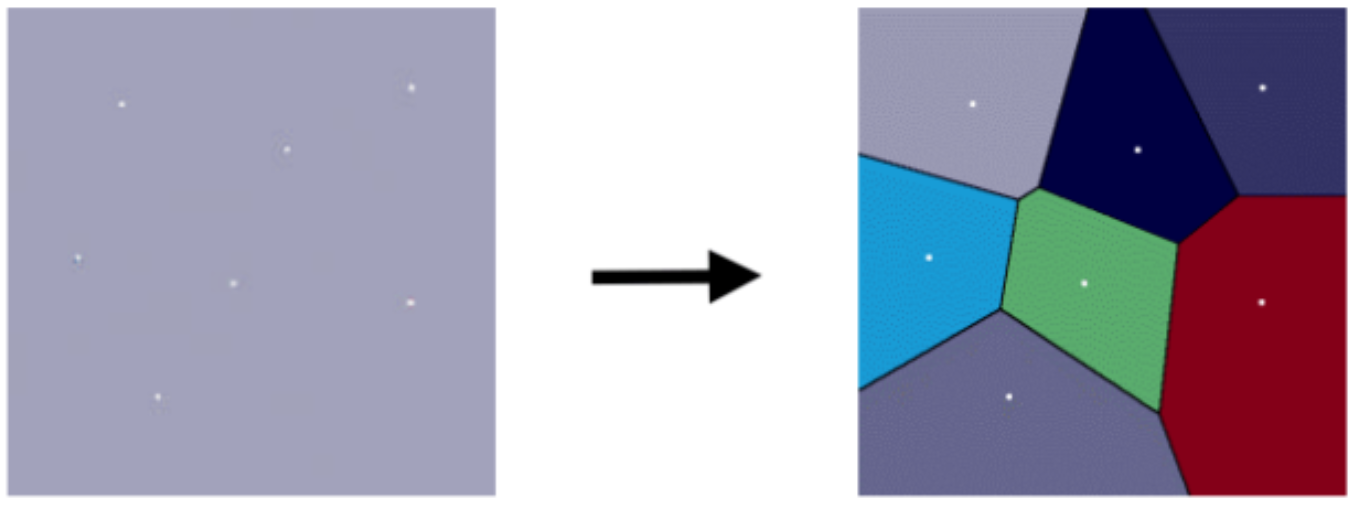
\includegraphics[scale=0.4]{Resources/PNG/Polygon.PNG}
		\caption{}
		\label{fig:PNG/Polygon.PNG}
	\end{center}
\end{figure}
Immer dann gut einsetzbar, wenn ungenaue Sensoren zur Verfügung stehen oder die Umwelt ungenau geometrisch modelliert wurde oder sich dynamisch ändert.
\paragraph{Generalisierte Voronoi-Diagramme}
\begin{itemize}
	\item Bei der Navigation von Robotern wird eine verallgemeinerte Version des Voronoi Diagramms verwendet, das sogenannte \textbf{generalisierte Voronoi Diagramm}(GVD)
	\item \textbf{Generalisierung} betrifft die \textbf{Form der Zentren} und die Art der \textbf{Abstandsfunktion}
	\item \textbf{Zentren} können aus \textbf{komplexeren Formen} wie Linien, Kurven oder Polygonen \textbf{statt Punkten} bestehen
	\item Objekten der Umgebung werden als \textbf{Voronoi-Zentren} behandelt
	\item Die Menge aller \textbf{Voronoi-Kanten}, das GVD, stellt mögliche \textbf{kollisionsfreie Wegstücke} dar
	\item Falls sich der Roboter entlang einer \textbf{Voronoi-Kante} bewegt, kann er nicht mit Hindernissen kollidieren
	\item Beliebtes Verfahren zur Repräsentation des Konfigurationsraumes und Erzeugung eines Graphen.
	\item Punkte an denen sich \textbf{Voronoi-Kanten} schneiden, werden zu \textbf{Voronoi-Knoten}
\end{itemize}
\begin{figure}[H]
	\begin{center}
		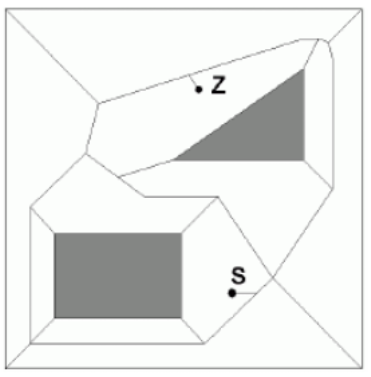
\includegraphics[scale=0.6]{Resources/PNG/Voronoi.PNG}
		\caption{}
		\label{fig:PNG/Voronoi.PNG}
	\end{center}
\end{figure}
Start- und Zielpunkt des gesuchten Weges liegen normalerweise nicht auf dem Diagramm.
Diese beiden Punkte werden mit der nächstliegenden Kante verbunden.
Die Berechnung des optimalen Weges auf dem Voronoi-Diagram kann mit üblichen Graphenalgorithmen vorgenommen werden.
\subsection{Navigation in einer Rasterkarte}
\begin{itemize}
	\item Die Karte ist durch ein binäres Raster mit freiem Platz und Hindernissen gegeben.
	\item Das Raster wird ausgehend vom Startpunkt: \textbf{geflutet} $\Rightarrow$ Füllt den gesamten Hindernisfreien Raum
	\item In jeder Iteration haben alle Pixel auf einer Wellenfront dieselbe Pfadlänge im Raster bezogen auf den Zielpunkt
	\item Backtracking vom Zielpunkt zurück zum Startpunkt und erstellt dabei eine Liste der passierten Rasterpunkte
	\item Gewählt kann jeder Punkt im Raster werden, dessen Wert eins geringer ist, als der aktuell betrachtete
	\item Trifft dies auf mehrere Punkte zu, wird willkürlich einer gewählt
\end{itemize}
\begin{figure}[H]
	\begin{center}
		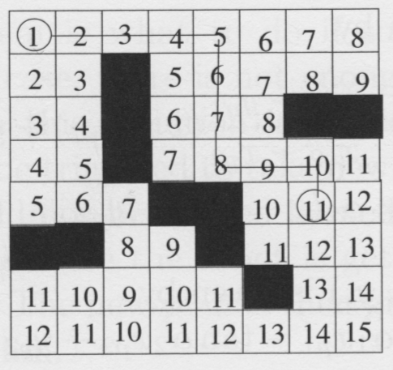
\includegraphics[scale=0.6]{Resources/PNG/RasterKarte.PNG}
		\caption{}
		\label{fig:PNG/RasterKarte.PNG}
	\end{center}
\end{figure}
\paragraph{Fluten der Karte}
\begin{itemize}
	\item Ein \textbf{Rasterpunkt} besitzt vier Nachbarpunkte: \enquote{N}, \enquote{O}, \enquote{S} , \enquote{W}
	\item Ein Rasterpunkt z ist mit 0 für freien Raum belegt und -1 für ein Hindernis
	\item Wenn ein Rasterpunkt eine Nummer erhalten hat, behält er diese Nummer
	\item Der Algorithmus benutzt aus Performancegründen zwei Stacks $S_0$ und $S_1$, die abwechselnd gefüllt und geleert werden. Die Stacks sind anfangs leer
\end{itemize}
\begin{figure}[H]
	\begin{center}
		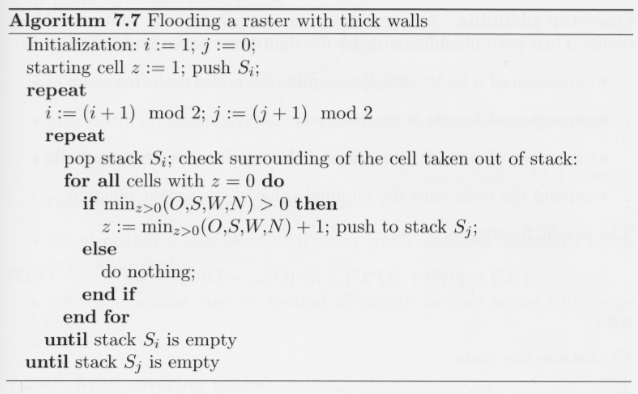
\includegraphics[]{Resources/PNG/Flooding.PNG}
		\caption{}
		\label{fig:PNG/Flooding.PNG}
	\end{center}
\end{figure}
\paragraph{Alternativer Wave Front Planer}
Siehe Ursprungsfolie Kapitel 5, Seite 29/30
\subsection{Potentialfeld methode}
\paragraph{Grundidee}
\begin{itemize}
	\item Vorbild: \textbf{Elektrisches Feld}
	\item Start- und Zielpositionen, die Positionen aller Hindernisse müssen bekannt sein.
	\item Der \textbf{Zielpunkt und Freiräume} erhalten ein \textbf{anziehendes Potential}
	\item Der \textbf{Startpunkt, die Hindernisse} und Wände erhalten ein \textbf{abstoßendes Potential}
	\item Es wird eine Karte generiert mit virtuell anziehenden und abstoßenden Kräften
	\item Kräfte nehmen linear mit dem Abstand zu den Objekten ab.
	\item \textbf{Ein Objekt bewegt sich nach der Methode des steilsten Abstiegs im Potentialfeld auf das Ziel zu.}
\end{itemize}
\begin{figure}[H]
	\begin{center}
		\includegraphics[scale=0.5]{Resources/PNG/Potentialfeld.PNG}
		\caption{}
		\label{fig:PNG/Potentialfeld.PNG}
	\end{center}
\end{figure}